% Rendu du sujet 3 (recuit simulé). Compiler avec : xelatex sujet3.tex (deux fois)
\documentclass[11pt,a4paper]{article}
\usepackage[a4paper,top=2.1cm,bottom=1.8cm,left=1.9cm,right=1.9cm,headsep=0.5cm]{geometry}
\usepackage[no-math]{fontspec}
\setmainfont{Inter}[Scale=0.88]
\setmonofont{DejaVu Sans Mono}[Scale=0.78]
\usepackage{polyglossia}\setmainlanguage{french}
\usepackage{amsmath,amssymb,icomma}
\usepackage{graphicx,xcolor,booktabs,tabularx,array,listings,fancyhdr,enumitem,tcolorbox}
\usepackage[hidelinks]{hyperref}

\definecolor{violet8}{HTML}{842577}
\definecolor{rouge8}{HTML}{E10717}
\definecolor{gris8}{HTML}{6B6B6B}
\definecolor{fond}{HTML}{F6F3F7}

\hypersetup{pdftitle={TP3 : Optimisation stochastique, le recuit simulé},
  pdfauthor={Esteban BERETTI--PRENANT},
  pdfsubject={Statistiques et Analyse de Données, Master Informatique I2A, Université Paris 8}}

\pagestyle{fancy}\fancyhf{}
\renewcommand{\headrulewidth}{0pt}
\fancyhead[L]{
\includegraphics[height=0.55cm]{paris8.png}}
\fancyhead[R]{\small\color{gris8}Statistiques et Analyse de Données · TP3}
\fancyfoot[C]{\small\color{gris8}\thepage\,/\,\pageref{fin}}

\newcommand{\barre}{{\color{violet8}\rule{0.55\linewidth}{0.6pt}}{\color{rouge8}\rule{0.45\linewidth}{0.6pt}}}
\newcommand{\question}[1]{\vspace{0.5em}{\large\bfseries\color{violet8}#1}\par\vspace{0.25em}}
\newcommand{\lecture}{{\bfseries\color{rouge8}Lecture.}\ }

\lstset{basicstyle=\ttfamily,keywordstyle=\color{violet8}\bfseries,commentstyle=\color{gris8},
  language=Python,columns=fullflexible,keepspaces=true,frame=none,backgroundcolor=\color{fond},
  xleftmargin=4pt,framexleftmargin=4pt,aboveskip=4pt,belowskip=4pt,
  literate={é}{{\'e}}1{è}{{\`e}}1{à}{{\`a}}1{ê}{{\^e}}1{π}{{$\pi$}}1{α}{{$\alpha$}}1}

\tcbset{coquille/.style={colback=rouge8!5,colframe=rouge8!70,boxrule=0.5pt,arc=2pt,
  left=5pt,right=5pt,top=3pt,bottom=3pt,fontupper=\small}}

\setlength{\parindent}{0pt}\setlength{\parskip}{0.35em}
\setlist{nosep,leftmargin=1.2em}

\begin{document}

% ---------- En-tête de la première page ----------
{\footnotesize\bfseries\color{rouge8}STATISTIQUES ET ANALYSE DE DONNÉES · RENDU}\par\vspace{0.2em}
{\LARGE\bfseries TP3 : Un algorithme d'optimisation stochastique, le recuit simulé}\par\vspace{0.2em}
{\color{violet8}Gradient simple (déterministe) contre recuit simulé (stochastique)}\par\vspace{0.3em}
\barre\par\vspace{0.1em}
{\small
\begin{tabularx}{\linewidth}{@{}>{\color{gris8}}l X >{\color{gris8}}l X@{}}
Auteur & Esteban BERETTI--PRENANT & Enseignant & M. Zerzeri\\
Formation & Master Informatique I2A, Université Paris 8 & Date & 18/11/2026\\
Outils & Python (numpy, scipy, matplotlib), graine 2026 & Notebook & \texttt{s3\_1\_recuit\_simule.ipynb}\\
Dépôt & \multicolumn{3}{l}{\href{https://github.com/Este34/presentation_statistique}{\color{violet8}github.com/Este34/presentation\_statistique} (code, tests, démonstrations complètes)}\\
\end{tabularx}}

\vspace{0.2em}
\textbf{Problème.} Minimiser $h(x) = x^2 + 3x\cos x$ sur $[-8\pi, 8\pi]$ en partant de
$x_0 = 7{,}5$, point situé dans le bassin d'attraction d'un minimum \emph{local} non global.
On compare le gradient simple, qui suit la pente, et le recuit simulé, qui accepte parfois de
remonter. (Maximiser $h$ reviendrait à minimiser $\tilde h = -h$.)

\question{Q1 · La fonction $h$ et ses extrema}
$h'(x) = 2x + 3\cos x - 3x\sin x$ et $h''(x) = 2 - 6\sin x - 3x\cos x$. Le terme $3x\cos x$
oscille avec une amplitude $3|x|$ croissante, et $h''$ change de signe ($h''(0) = 2 > 0$,
$h''(2\pi) = 2 - 6\pi < 0$) : $h$ \textbf{n'est pas convexe}. De plus $h(x) \ge x^2 - 3|x| = |x|(|x| - 3) > 0$ pour $|x| > 3$, alors que $h$ prend
des valeurs négatives : le minimum global est forcément dans $]-3, 3[$.

\begin{center}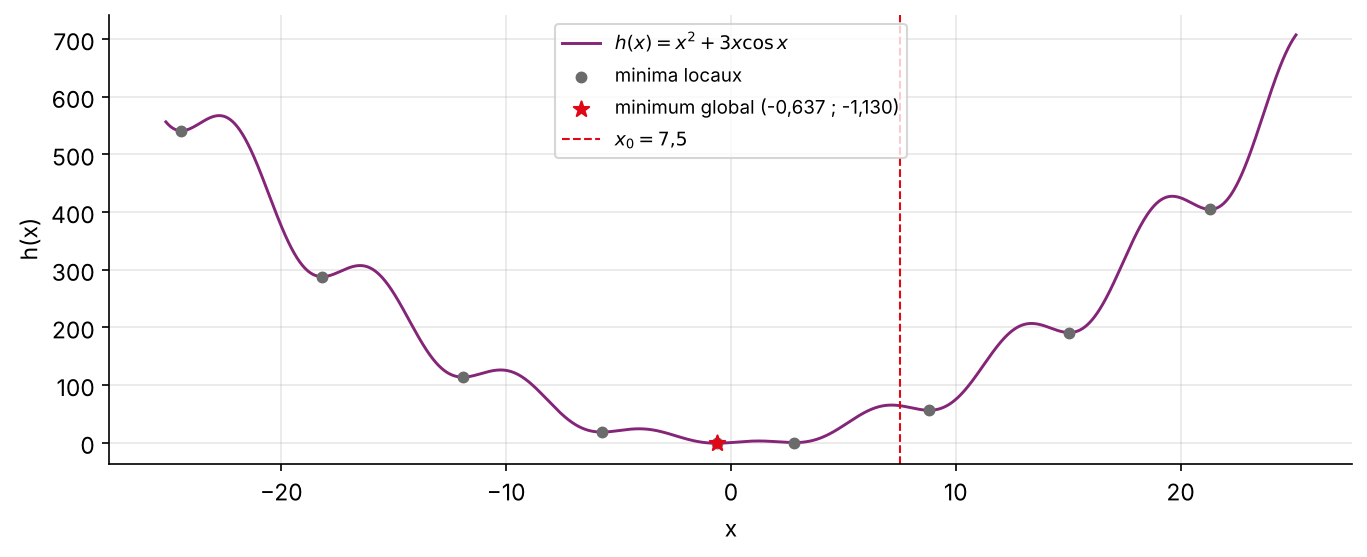
\includegraphics[width=0.86\linewidth]{../../sujets/sujet3/figures/s31_h.png}\end{center}
\vspace{-0.6em}
\lecture Sur 5000 points, \texttt{min} donne $h(-0{,}6385) = -1{,}1304$ ; en affinant le zéro
de $h'$ : minimum global $x^\star = -0{,}6371$, $h(x^\star) = -1{,}1305$. On compte
\textbf{9 minima locaux}. Le plus traître est $x = 2{,}805$ ($h = -0{,}075$), presque aussi bas que
le global. $x_0 = 7{,}5$ est entre les maxima $7{,}14$ et $13{,}37$ : dans le bassin du minimum
local $8{,}814$ ($h = 56{,}03$).

\begin{tcolorbox}[coquille]
\textbf{Coquilles de l'énoncé.} (1) « $h = -h$ » : lire $\tilde h = -h$. (2) Avec
$y_n = -8\pi + 16\pi\,\frac{n-1}{5000}$, le dernier point vaut $25{,}1227 < 8\pi = 25{,}1327$ :
diviser par 4999, comme \texttt{linspace}. (3) La lettre $\alpha$ désigne à la fois le pas
$\alpha_n$ du gradient et le facteur de refroidissement $0{,}99$ du recuit. (4) « $\alpha_n = O(1/n)$ »
ne suffit pas à avoir $\sum\alpha_n = +\infty$ ($1/n^2$ est un $O(1/n)$) : il faut
$\alpha_n \propto 1/n$. (5) $\alpha_0 = 0{,}025/0$ n'est pas défini : on numérote
$x_n = x_{n-1} - \alpha_n h'(x_{n-1})$ pour $n \ge 1$ (de même, le pas $n$ du recuit utilise $T_n$).
(6) Le recuit vise les \emph{minima} globaux, et la convergence est en probabilité, pas presque
sûre (Q4).
\end{tcolorbox}

\question{Q2 · Gradient simple}
$x_n = x_{n-1} - \alpha_n h'(x_{n-1})$, $\alpha_n = 0{,}025/n$ : $\sum\alpha_n = +\infty$ (on peut
aller aussi loin que nécessaire) et $\sum\alpha_n^2 < \infty$ (les pas s'éteignent). Par Taylor,
$h(x - \alpha_n h'(x)) \le h(x) - \alpha_n h'(x)^2\,(1 - \alpha_n M/2)$ avec $M \ge h''$ sur le
segment parcouru ; ici $M \approx 20{,}2$ et $\alpha_n \le 0{,}025$, donc $\alpha_n M/2 < 1$ : $h$
baisse strictement à chaque pas.
\noindent\begin{minipage}{\linewidth}
\begin{lstlisting}
def gradient_simple(grad, x0, N, pas=lambda n: 0.025 / n):
    x = np.empty(N + 1); x[0] = x0
    for n in range(1, N + 1):
        x[n] = x[n - 1] - pas(n) * grad(x[n - 1])   # x_n = x_{n-1} - α_n h'(x_{n-1})
    return x
\end{lstlisting}
\end{minipage}
\begin{center}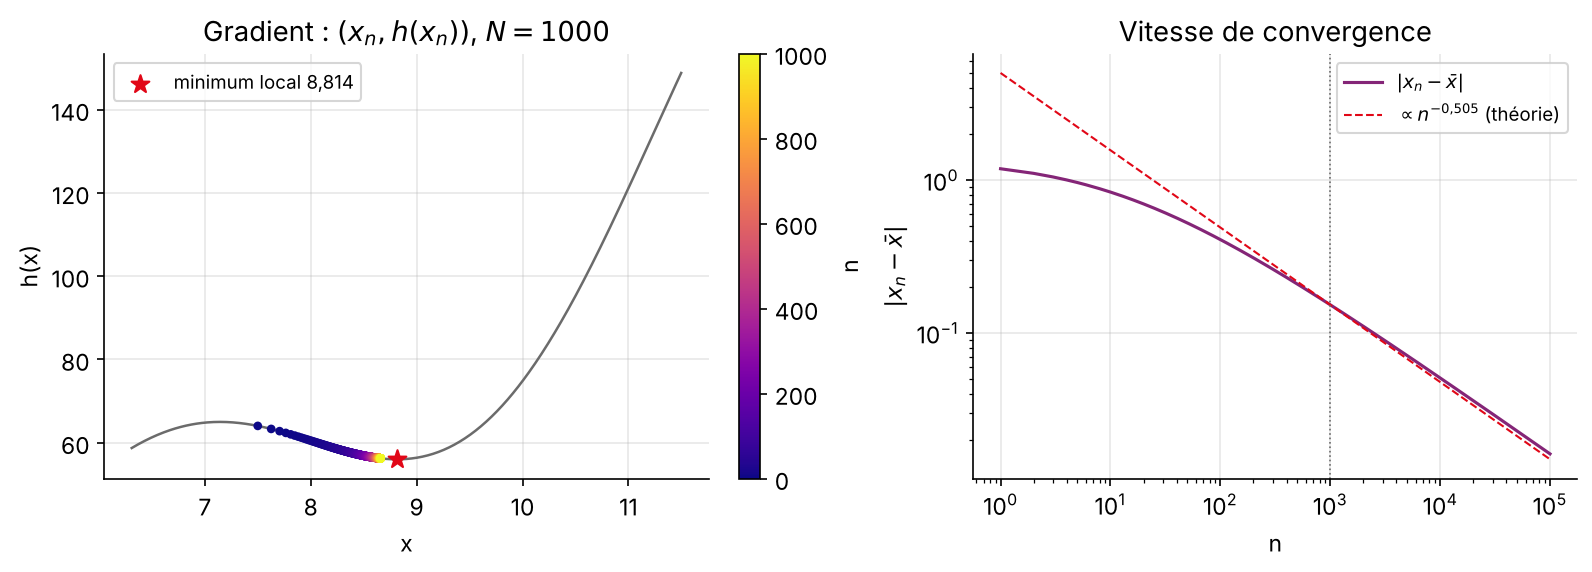
\includegraphics[width=0.93\linewidth]{../../sujets/sujet3/figures/s32_gradient.png}\end{center}
\vspace{-0.6em}
\lecture $h'(7{,}5) = -5{,}07 < 0$ : la suite part vers la droite, $h$ décroît à chaque pas, et
après 1000 itérations $x_N = 8{,}661$ ($h = 56{,}25$). Le gradient \textbf{converge vers le
minimum local} $8{,}814$, jamais vers le global : il ne peut pas remonter le col en $7{,}14$.
La convergence est \textbf{lente}. Notons $\bar x = 8{,}814$ ce minimum local et
$e_n = x_n - \bar x$ l'erreur. Comme $h'(x) \approx h''(\bar x)(x - \bar x)$,
$e_{n+1} \approx (1 - c/n)\,e_n$ avec $c = 0{,}025\,h''(\bar x) = 0{,}505$, d'où
$|e_n| \approx C n^{-c}$ ($C$ constante). On mesure
$|e_n| = 0{,}153$ ; $0{,}051$ ; $0{,}016$ pour $n = 10^3, 10^4, 10^5$, soit une pente log-log de
$-0{,}494$ pour $-0{,}505$ prévu : l'erreur décroît en $1/\sqrt n$.

\question{Q3 · Recuit simulé}
On propose $z \sim \mathcal U[x_n - \frac\pi2, x_n + \frac\pi2]$ et on l'accepte avec la
probabilité $\min(1, e^{-\Delta h_n / T_n})$, $\Delta h_n = h(z) - h(x_n)$, avec
$T_n = 500 \times 0{,}99^n$. En pratique on tire $U \sim \mathcal U[0,1]$ et on accepte si
$U < e^{-\Delta h_n/T_n}$, puisque $P(U < p) = p$. Choix d'implémentation : un $z$ hors de
$[-8\pi, 8\pi]$ est refusé.
\begin{lstlisting}
for n in range(1, N + 1):
    T = T0 * alpha**n                                   # température T_n
    z = x[n - 1] + rng.uniform(-np.pi / 2, np.pi / 2)  # loi instrumentale g_n
    u = rng.random()
    if a <= z <= b and (h(z) <= h(x[n-1]) or u < np.exp(-(h(z) - h(x[n-1])) / T)):
        x[n] = z                                        # z accepté
    else:
        x[n] = x[n - 1]                                 # z refusé
\end{lstlisting}
\begin{center}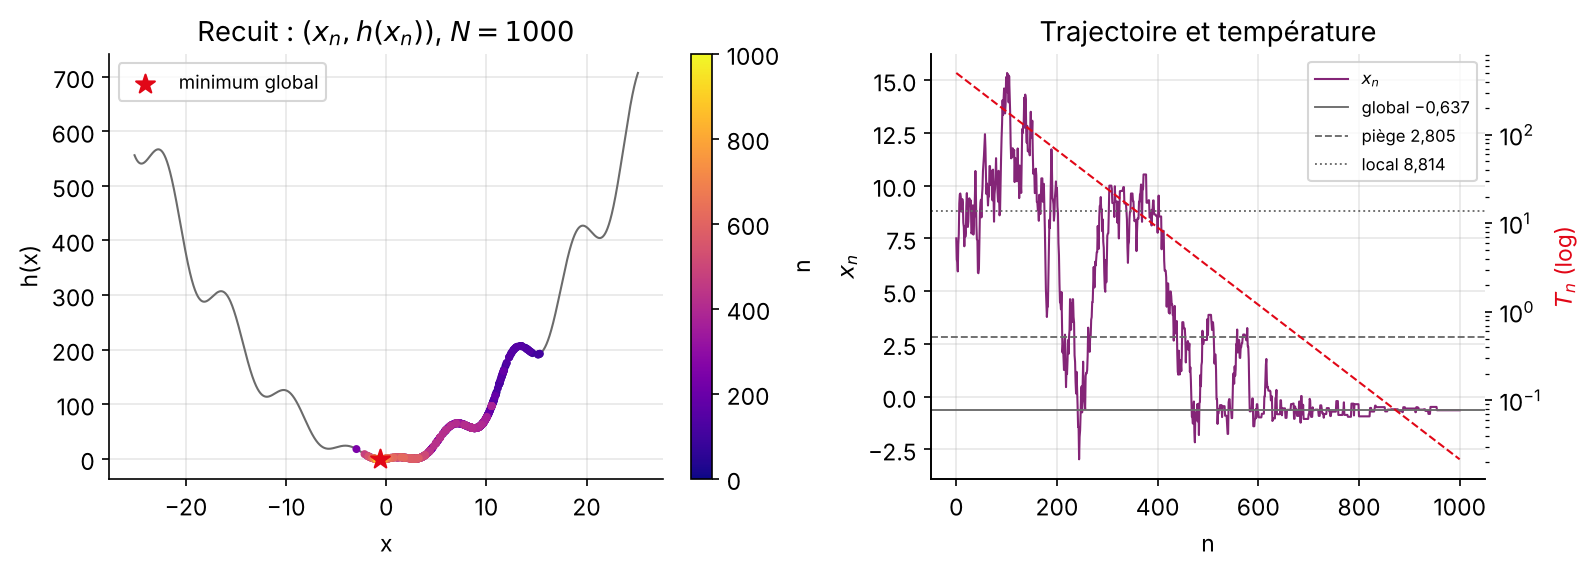
\includegraphics[width=0.93\linewidth]{../../sujets/sujet3/figures/s33_recuit.png}\end{center}
\vspace{-0.6em}
\lecture Partant du même $x_0 = 7{,}5$, la trajectoire \textbf{sort du bassin local} : à haute
température presque tout est accepté (taux de $0{,}99$ sur les 100 premières itérations) et la
suite explore $[-3 ; 15{,}3]$. Quand $T_n$ passe sous 1 ($n \approx 618$), elle se fixe progressivement : dernière
sortie du voisinage $\pm 0{,}5$ de $x^\star$ à $n = 702$, taux d'acceptation final $0{,}09$.
Résultat : $x_N = -0{,}650$, $h(x_N) = -1{,}1298$ contre $-1{,}1305$ : le \textbf{minimum
global} est trouvé, avec une précision limitée par la largeur fixe ($\pm\pi/2$) des propositions.

\emph{Pourquoi le global ?} À $T$ fixé, la proposition est symétrique et la chaîne vérifie
l'équilibre détaillé pour la loi de Boltzmann $\mu_T(x) \propto e^{-h(x)/T}$. Or
$\mu_T(x)/\mu_T(x^\star) = e^{-(h(x) - h(x^\star))/T} \to 0$ quand $T \to 0$ : la loi
stationnaire se concentre sur les minima globaux.

\question{Q4 · Comparaison et commentaires}
Un lancer du recuit est un résultat aléatoire : on le relance $R = 1000$ fois et on estime la
proportion de succès $\hat p$ avec son erreur-type $\sqrt{\hat p(1-\hat p)/R}$.
\begin{center}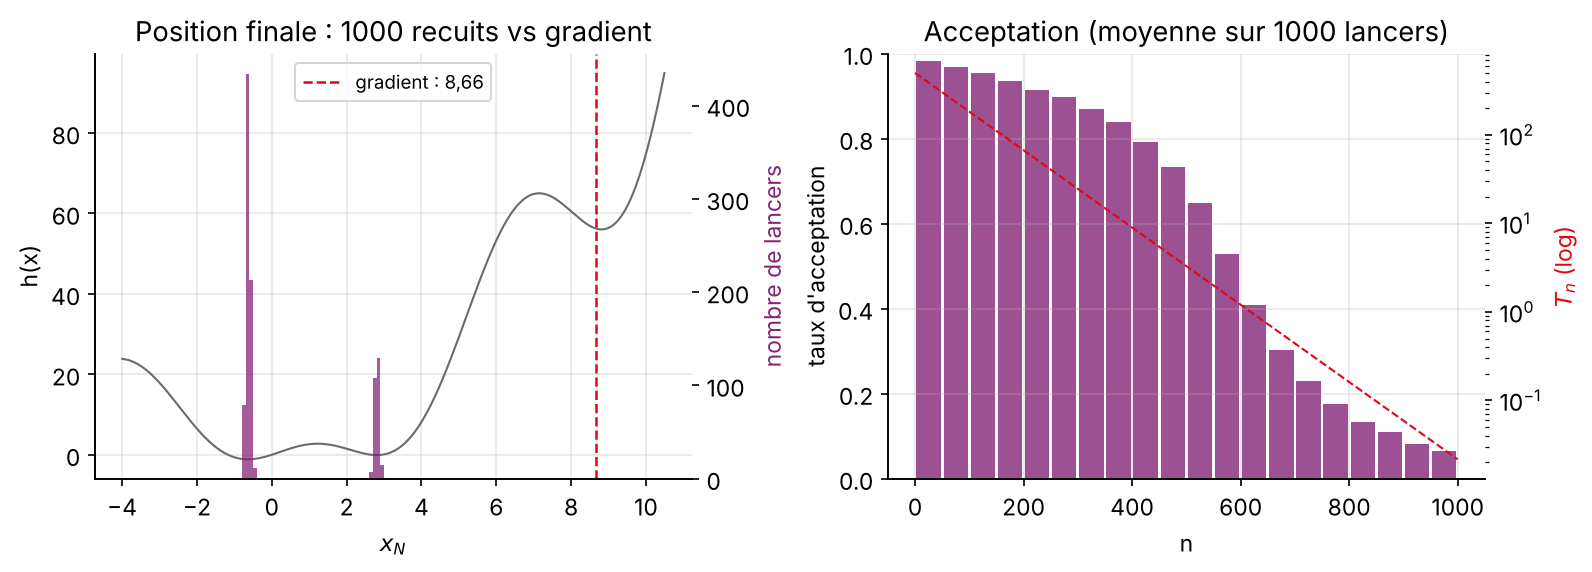
\includegraphics[width=0.93\linewidth]{../../sujets/sujet3/figures/s34_comparaison.png}\end{center}
\vspace{-0.6em}
\lecture Le gradient finit toujours en $8{,}66$ (0 succès). Le recuit atteint le minimum global
dans \textbf{73,8~\%~±~2,7~\%} des lancers (IC à 95~\%) et reste piégé en $2{,}805$ dans
\textbf{25,9~\%} des cas. L'affirmation de l'énoncé (« ce choix garantit la convergence presque
sûre ») est \textbf{fausse} : avec $T_n = T_0\alpha^n$, $\sum_n e^{-d/T_n} < \infty$ pour toute
hauteur de col $d > 0$ (moins de $10^{-30}$ au-delà de $n = 1000$ pour $d = 1{,}5$), donc la
chaîne ne franchit presque sûrement plus qu'un nombre fini de cols (Borel-Cantelli) : elle
\emph{gèle}, et ces 25,9~\% sont la proportion limite. La garantie théorique (Hajek, 1988, espace
fini) est une convergence \emph{en probabilité}, avec $T_n = c/\ln n$ et $c$ au moins égal à la
profondeur du minimum local non global le plus profond ($\approx 26$ pour de petits pas,
$\approx 12$ avec des sauts de $\pm\pi/2$) : beaucoup trop lent en pratique. Intuition du 25~\% :
les deux minima les plus bas ne diffèrent que de $1{,}06$ ; la chaîne gèle vers $T \approx 1$, où
la loi de Boltzmann met $\approx 25$~\% de sa masse dans le bassin de $2{,}805$. Refroidir plus lentement ($\alpha = 0{,}995$, $N = 2000$, 400 lancers) donne
77,0~\%~±~4,1~\%, écart de 1,27 erreur-type : \textbf{non significatif}.

\vspace{0.3em}
{\small
\renewcommand{\arraystretch}{1.25}
\begin{tabularx}{\linewidth}{@{}>{\bfseries\leavevmode\color{violet8}}p{2.9cm} X X@{}}
\toprule
 & \textbf{Gradient simple} & \textbf{Recuit simulé} \\ \midrule
Garantie & Minimum \textbf{local}, celui du bassin de $x_0$ ; global garanti si $h$ convexe (ou si $x_0$ est dans le bassin du global) &
Global en probabilité si $T_n = c/\ln n$ ($c$ assez grand) ; aucune avec $T_n = T_0\alpha^n$ (74~\% ici) \\
Vitesse & $|e_n| \approx C n^{-0,5}$ ici ; géométrique avec un pas constant &
Bon bassin atteint vers $n \approx 700$ ; précision finale grossière \\
Coût & 1 évaluation de $h'$ par itération ; un seul lancer suffit (déterministe) &
1 évaluation de $h$ et 2 tirages par itération ; plusieurs lancers pour juger le résultat \\
Compréhension & Simple : on descend la pente &
Plus subtile : chaîne de Markov, loi de Boltzmann, refroidissement \\
Mise en œuvre & 1 paramètre (le pas), mais il faut $h'$ &
3 réglages ($T_0$, $\alpha$, largeur de $g_n$), pas besoin de $h'$ \\
\bottomrule
\end{tabularx}}

\vspace{0.4em}
\textbf{Conclusion.} Le gradient est simple, peu coûteux et reproductible, mais lent ici et prisonnier du bassin de
$x_0$. Le recuit échappe aux minima locaux au prix de réglages délicats et d'un résultat
aléatoire. En pratique on les combine : recuit pour explorer, puis gradient depuis le meilleur
point visité pour affiner, ou plusieurs recuits indépendants (avec 2 lancers, l'échec tombe à
$0{,}262^2 \approx 7$~\%).
\label{fin}
\end{document}
